
%-------------------------------------------------------------------------%
\section{Masses of stop particles}


%\begin{align}
%    \begin{pmatrix} \Tilde{t}_1 \\ \Tilde{t}_2 \end{pmatrix} = 
%    \begin{pmatrix} \cos\theta_\Tilde{t} & -\sin\theta^*_\Tilde{t} \\ \sin\theta_\Tilde{t} & \cos\theta^*__\Tilde{t} \end{pmatrix}
%    \begin{pmatrix} \Tilde{t}_L \\ \Tilde{t}_R \end{pmatrix}
%    \label{eq:stopMass}
%\end{align}

%\begin{align}
%    \mathbf{m^2_\Tilde{t}} =
%    \begin{pmatrix}
%    m^2_{Q_3} + m^2_t + \Delta_{\Tilde{u}_L} & v(a^*_t\sin\beta - \mu y_t \cos\beta) \\
%    v(a_t\sin\beta - \mu^2 y_t \cos\beta) & m^2_{\Bar{u}_3} + m^2_t + \Delta_{\Tilde{u}_R}
%    \end{pmatrix}
%    \label{eq:stopMatrix}
%\end{align}

Here, the terms not yet mentioned are \cite{martin1997supersymmetry, arbey2012higgs}:
\begin{itemize}
  \item $m^2_{t}$ = squared mass of the top quark
  \item $m^2_{Q_3}$ = squared mass of the third-family squark
  \item $ m^2_{\Bar{u}_3}$ = squared mass of the third-family sleptons
  \item $\Delta_{\Tilde{u}_L/R}$ = contribution from the sleptons to the mass
  \item $a_t$ = soft scalar coupling term
  \item $v$ = vacuum expectation value (VEV) of the Higgs
  \item $\mu$ = Higgs-Higgsino mass parameter
  \item $\beta$ = VEV coupling angle. By convention, $0 < \beta < \pi/2$
\end{itemize}

%-------------------------------------------------------------------------%
\section{Possible decay channels of the top squarks} \label{sec:stopDecay}





\begin{figure}[htbp]
    \centering
    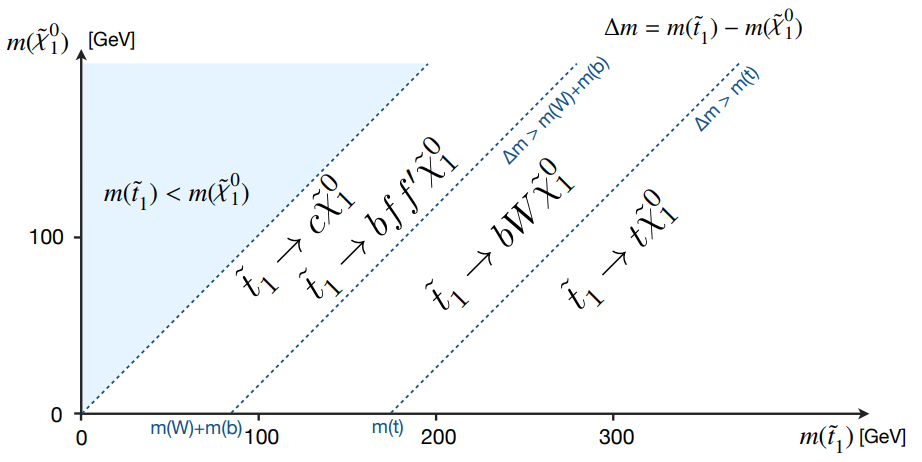
\includegraphics[width=15cm, height= 7.5cm]{decaymodes.png}
    \caption{Possible decay modes for stops within the mass-parameter-space of $\Tilde{t}_1 $ and $ \Tilde{\chi}_1^0 $ \cite{aad2014search}.}
    \label{fig:decayMode}
\end{figure}